\documentclass[12pt,letterpaper]{article}
\usepackage{natbib}

%Packages
\usepackage{pdflscape}
\usepackage{fixltx2e}
\usepackage{textcomp}
\usepackage{fullpage}
\usepackage{float}
\usepackage{latexsym}
\usepackage{url}
\usepackage{epsfig}
\usepackage{graphicx}
\usepackage{amssymb}
\usepackage{amsmath}
\usepackage{mathtools}
\usepackage{bm}
\usepackage{array}
\usepackage[version=3]{mhchem}
\usepackage{ifthen}
\usepackage{caption}
\usepackage{hyperref}
\usepackage{amsthm}
\usepackage{amstext}
\usepackage{enumerate}
\usepackage[osf]{mathpazo}
\usepackage{dcolumn}
\usepackage{lineno}
\usepackage{dcolumn}
\usepackage{mathtools}

\DeclarePairedDelimiter\abs{\lvert}{\rvert}%
\DeclarePairedDelimiter\norm{\lVert}{\rVert}%
\newcolumntype{d}[1]{D{.}{.}{#1}}

\pagenumbering{arabic}


%Pagination style and stuff
\linespread{2}
\raggedright
\setlength{\parindent}{0.5in}
\setcounter{secnumdepth}{0} 
\renewcommand{\section}[1]{%
\bigskip
\begin{center}
\begin{Large}
\normalfont\scshape #1
\medskip
\end{Large}
\end{center}}
\renewcommand{\subsection}[1]{%
\bigskip
\begin{center}
\begin{large}
\normalfont\itshape #1
\end{large}
\end{center}}
\renewcommand{\subsubsection}[1]{%
\vspace{2ex}
\noindent
\textit{#1.}---}
\renewcommand{\tableofcontents}{}
%\bibpunct{(}{)}{;}{a}{}{,}

%---------------------------------------------
%
%       START
%
%---------------------------------------------

\begin{document}

%Running head
\begin{flushright}
Version dated: \today
\end{flushright}
\bigskip
\noindent RH: Characters correlation

\bigskip
\medskip
\begin{center}

\noindent{\Large \bf Effect of discrete character correlation on tree inference}
\bigskip

\noindent {\normalsize \sc Thomas Guillerme$^1$$^*$, and Martin D. Brazeau$^1$}\\
\noindent {\small \it 
$^1$Imperial College London, Silwood Park Campus, Department of Life Sciences, Buckhurst Road, Ascot SL5 7PY, United Kingdom.\\}
\end{center}
\medskip
\noindent{*\bf Corresponding author.} \textit{t.guillerme@imperial.ac.uk}\\ 
\vspace{1in}

%Line numbering
\modulolinenumbers[1]
\linenumbers

%---------------------------------------------
%
%       ABSTRACT
%
%---------------------------------------------

\newpage
\begin{abstract}
blablabla
\end{abstract}

\noindent (Keywords: )\\

\vspace{1.5in}

\newpage 


%---------------------------------------------
% LaTeX tips for modifying/editing the document:
%---------------------------------------------
% - You can comment using the percentage sign. I suggest you use the % sign alone for commenting out sections of the text:
%       e.g. "This is a really long sentence %because this sentence is very long." Here the % is used for ignoring the end of the sentence (but for some reason you want to keep track of it).%
%       For comments as in verbose comments, I suggest you use "%MB:":
%       e.g. "This is a really long sentence %because this sentence is very long. %MB: yeah, no shit!" 
% - For optimal version control, write only one sentence per line (for more precise track changes)
% - To build the pdf, use command+B in Sublime.
% - Because of the bibliography, the pdf needs to be build in the same folder that contains "References.bib" and "sysbio.bst"
% - For citing papers, you must put their bibtex reference in the "References.bib" file and then you can use the following sysbio tags:
%        \cite{bibtexBob2000} for citing within a sentence: "Bob (2000)"
%        \citep{bibtexBob2000} for citing within brackets: "(Bob, 2000)"
%        \citep[Before:][-After]{bibtexBob2000} for citing within brackets with additional text: "(Before: Bob, 2000 -After)"
%        \citealt{bibtexBob2000} for citing without brackets: "Bob, 2000"
%        You can put more cites in each \cite tag by separating them with commas.
% - For equation, find every details here: https://en.wikibooks.org/wiki/LaTeX/Mathematics
% - For titles and stuff, the hierarchy goes \section{}, \subsection{}, \subsubsection{} and so forth...
% - For bullet points or enumerations you can use:
%       \begin{itemize}
%           \item my first bullet point/enumeration
%       \end{itemize}
%       With replacing "itemize" by "enumerate" for enumeration.




%---------------------------------------------
%
%       INTRODUCTION
%
%---------------------------------------------
\section{Introduction}

The last five years have seen a drastic expansion of the use of discrete morphological data in macroevolutionary studies.
In fact, traditionally confined to ``classic'' cladistics \citep{felsenstein2004inferring}, these methods have recently been expended and improved whether based on the models and methods for inferring phylogenies \citep{lewisa2001,Wright01072016} or the methods to date them \citep[e.g.][]{bapsta2013} or to combine them with molecular data \citep{pyrondivergence2011,ronquista2012}.
% Debate on which inference method to use \citep{spencerefficacy2013,wrightbayesian2014,OReilly20160081}.
% Debate on dating methods \citep{Arcila2015131}.
% Debate on data sources (BAPST in review)
In parallel, much development has also been done on pre-phylogenetic analysis \citep[e.g. data collection;][]{morphobank} as well as on post-phylogenetic analysis \citep[e.g. morphological disparity analysis;][]{Close2015,Claddis}.
However, using discrete morphological data in macroevolutionary studies comes with several caveats based to the nature of data used \citep{Guillerme2016146}(+BAPST); the coding of this data \citep{Brazeau2011}; the inference \citep{spencerefficacy2013,wrightbayesian2014,OReilly20160081} or the dating methods \citep{Arcila2015131}.

However, one aspect of the data is often neglected: the correlation that exists between discrete morphological characters.
In fact, because of their nature, these characters are prone to many sources of correlation such as: (1) the co-evolution between traits (e.g. the number of digits on a limb co-evolves with the actual presence/absence of the limb); (2) morphological modularity \citep[i.e. the unity of entire morphological regions][]{goswami2006morphological}; (3) convergent evolution between traits (e.g. wings in many vertebrates); or (4), more down-to-earth, to errors from the coder \citep[e.g. the repetition of the same character described slighlty differently each case][]{Brazeau2011}.
These sources of correlation can alter the results of phylogenetic inference by effectively weighting the correlated characters against their non-correlated counter parts leading to biases in phylogenetic inference by supporting clades with artificial synapomorphies.
This fact have led to the popular wisdom rule of avoiding coding correlated characters for macroevolutionary studies.

Up to this date, a lot of work has been done on character correlation \textit{per se}, but focussing mainly on how to measure correlation between characters to detect patterns of coevolution \citep{Lande1983,Maddison1990,Pagel1994,Pagel2006,Grabowski2016}.

Also \cite{goswami2010}.

However, only several attempts have been made on the actual effect of characters correlation on phylogenetic inference with two notable exceptions of \cite{Davalos01072014} on empirical data and \cite{ZouConvergence} on molecular data.
It is thus still unclear what will be the effect of characters correlation on phylogenetic inference: how does these correlation really affect topology?
Additionally, because of the nature of discrete morphological characters and organisms morphology, correlation is expected to rise through both combinatorics properties of the characters or simply through evolutionary processes.
What is the effect of these two sources of correlations and can we (should we) avoid them?

In this study, we formally assess the effect of discrete character's correlation using simulated and empirical data.
We propose a new metric to measure the correlation (or difference) between two discrete characters and a protocol to modify discrete data matrices to increase/decrease the correlation between characters within/
We found that blabalbal

\section{Methods}

We applied the following simulation protocol to assess the effect of characters correlation (Fig.\ref{Fig:outline}):
\begin{enumerate}
    \item \textbf{Simulating matrices}: we simulated discrete morphological matrices with 25, 75 and 150 taxa for 100, 350 and 1000 characters, hereafter called the ``normal'' matrices.
    \item \textbf{Modifying matrices}: we modified the ``normal'' matrices by duplicating characters in order to maximise and minimise characters differences (hereafter called respectively ``maximised'' and ``minimised'' matrices) by removing respectively the least or most different characters and replacing them randomly by the remaining characters. We also randomly duplicated characters from the ``normal'' matrices without biasing towards maximised or minimised character difference to create null expectancy matrices (hereafter called the ``null'' matrices).
    \item \textbf{Inferring topologies}: we inferred the topologies from the ``normal'', ``maximised'', ``minimised'' and ``null'' matrices using both Maximum Parsimony and Bayesian inference (hereafter called the ``normal'', ``maximised'', ``minimised'' and ``null'' trees).
    \item \textbf{Comparing topologies}: finally, we compared to topologies in two ways: (1) first we compared the ``normal'' to the ``null'' trees to assess our simulation protocol; (2) second, we compared the ``maximised'' and ``minimised'' trees to the ``null'' and ``normal'' trees respectively to measure the signal to noise ratio and thus measure the effect of character correlation on topology.
\end{enumerate}
Each steps are described below in more details, as well as our proposed definition of the Character Difference metric.


\begin{figure}[!htbp]
\centering
   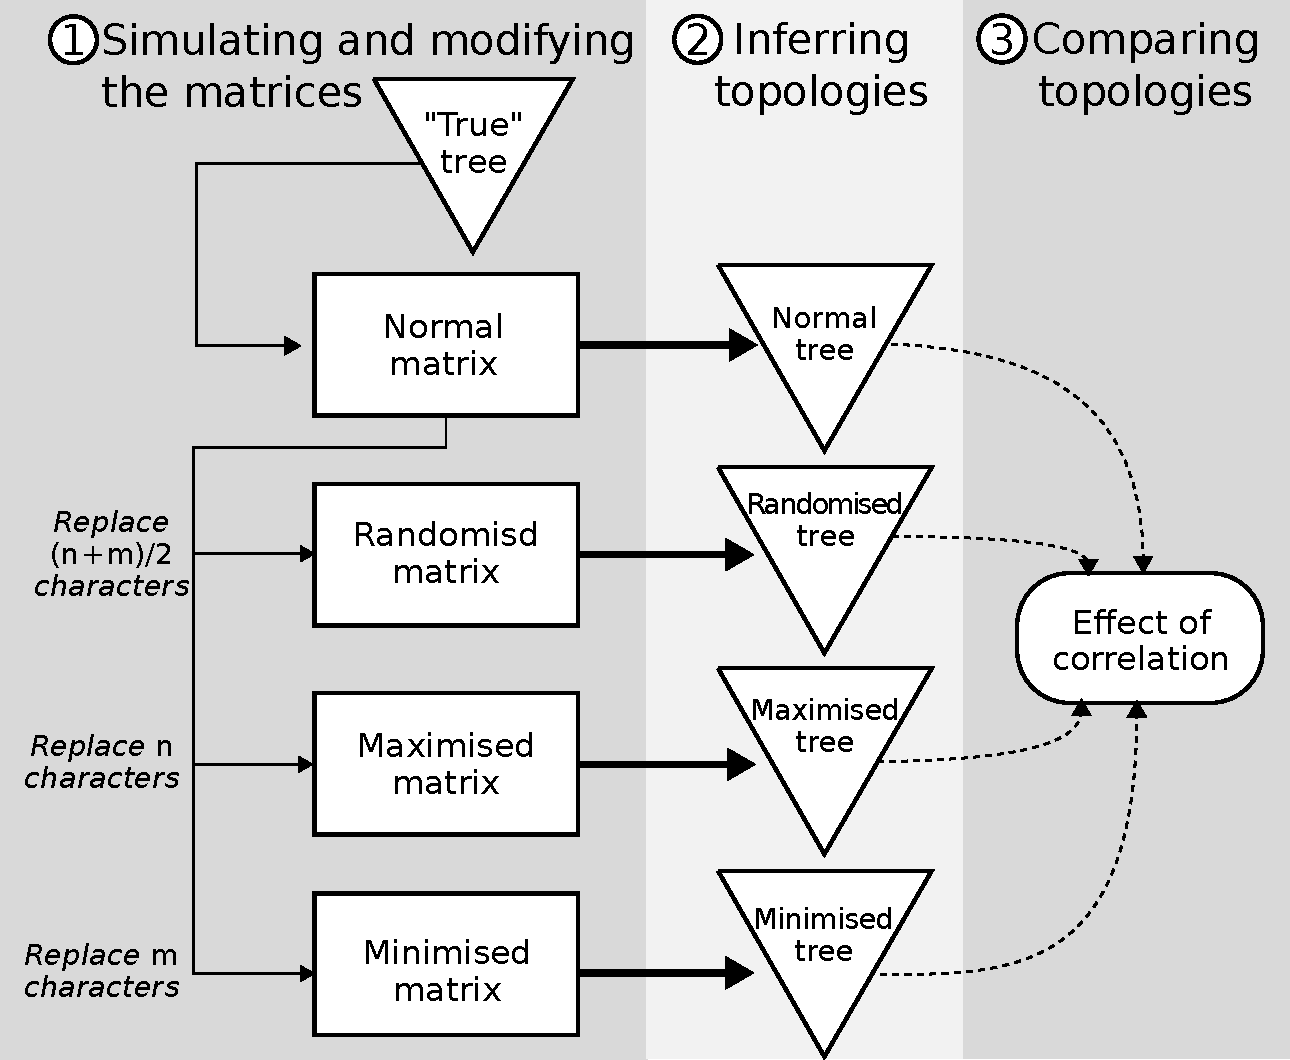
\includegraphics[width=0.9\textwidth]{Figures/outline.pdf}
\caption{Outline of the simulation protocol: the first step includes both the simulation and the modification of the matrices (thin solid lines); the second step includes tree inference using Maximum Parsimony and Bayesian inference (thick solid lines); the third step includes comparing the resulting tree topologies (dashed lines).}
\label{Fig:outline}
\end{figure}


\subsection{Measuring correlation between characters}
We define characters as being correlated if they give the same phylogenetic information.
In order to measure this similitude in phylogenetic information, we propose a new distance metric to measure the difference between two characters:

\subsubsection{Characters difference (CD)}
\begin{equation}
    CD_{(x,y)} = 1 - \left(\frac{\abs*{\frac{\sum_{i}^{n}\abs{x_{i} - y_{i}}}{n}-\frac{1}{2}}}{\frac{1}{2}}\right)
\end{equation}

\noindent Where $n$ is the number of taxa with comparable data and $x_i$ and $y_i$ are each characters states for the characters $x$ and $y$ and the taxa $i$.
$CD$ is a continuous distance metric valid in a mathematical sense (see Supplementary).
Since we are considering differences as being only Fitch-like (i.e. non-weighted and non-ordinate), we ignore the actual distance between two different character states tokens \citep[i.e. a Gower distance;][]{GowerDist}.
Two same character states tokens have a difference of $0$ and two different ones have a difference of $1$ (e.g. $0 - 0 = 0$ or $1 - 8 = 1$).
In order to facilitate and standardise characters states comparison, we standardised each characters by arbitrarily modifying their character states tokens by order of appearance.
In other words, we replaced all the occurrences of the first token to be $0$, the second to be $1$, etc.
This way, a character \texttt{A = \{2,2,3,0,0,3\}} would be standardised as \texttt{A' = \{0,0,1,2,2,1\}} \citep[following the \textit{xyz} notation in][p.13]{felsenstein2004inferring}.
Note that in terms of phylogenetic signal, both \texttt{A} and \texttt{A'} are exactly identical (forming three distinct groups).
When the character difference is equal to $0$, it means that characters convey the same phylogenetic signal.
When the character difference is equal to $1$ it means it conveys the most different signal.
For example with three characters \texttt{A = \{0,1,1,1\}}, \texttt{B = \{1,0,0,0\}} and \texttt{C = \{0,1,2,3\}}, $CD_{(A,B)} = 0$ and $CD_{(A,C)} = 1$.

\subsection{Simulating discrete morphological matrices}
To simulate the matrices we applied a protocol very similar to \citep{Guillerme2016146}.
First, we generate random birth-death trees with the birth ($\lambda$) and death ($\mu$) parameters sampled from a uniform ($0$,$1$) distribution maintaining $\lambda$ $>$ $\mu$ using the diversitree \texttt{R} package \citep[v0.9-8;][]{fitzjohndiversitree2012} and saving the tree after reaching either 25, 75 or 150 taxa.
For each tree, we arbitrarily set the outgroup to be the first taxa (alphabetically) thus effectively rooting the trees on this taxa.
These trees are hereafter called the ``true'' trees.
We then simulated discrete morphological characters using the either of the two following models:
\begin{itemize}
    \item The HKY-binary model \citep{OReilly20160081} which is an HKY model \citep{HKY85} with a random states frequency (sampled from a uniform distribution $(0,1)$ an scale to sum to one) and using a transition/transvertion rate of two \citep{douadycomparison2003} but where the purines (A,G) were changed into state $0$ and the pyrimidines (C,T) in state $1$.
    This model has the advantage of not favouring Bayesian inference \citep[since it doesn't use a M$k$ model;][; see below]{OReilly20160081} but the downside of it is it can only generate binary state characters \citep[or 4 states;][]{puttick2017uncertain}.
    \item To generate more than binary states characters, we used the M$k$ model \citep{lewisa2001}.
    We draw the number of character states with a probability of $0.85$ for binary characters and $0.15$ for three state characters \citep{Guillerme2016146}.
    This model assumes a equal transition rate between character states that might seem overly simplifying and excludes other observed transition patterns \citep[e.g. Dollo characters;][]{Dollo,wright2015came}.
    Recently however, \cite{Wright01072016} have shown that an equal rate transition is still strictly majority in empirical data.
\end{itemize}

\noindent For each character, both models (HKY-binary or M$k$) where chosen randomly and ran with an overall evolutionary rate drawn from a gamma distribution ($\beta$ = $100$ and $\alpha$ = $5$).
This low evolutionary rate values allowed to reduce the number of homoplasic character changes and thus reinforce the phylogenetic information in the matrices (see supplementary materials @@@).
We re-simulated every invariant characters to obtain a matrix with no invariant characters.
To ensure that our simulation where reflecting realistic observed parameters, we only selected matrices with Consistency Indices superior to $0.26$ \citep{OReilly20160081}.

For each trees with 25, 75 or 150 taxa we generated matrices with 100, 350 and 1000 characters following \cite{OReilly20160081}.
The matrices where generated using the \texttt{dispRity R} package \citep[][; \url{https://github.com/TGuillerme/dispRity}]{thomas_guillerme_2016_55646}.
To estimate the variance of our simulations and assess the effect of our random parameters, we repeated this step 50 times resulting in 450 morphological matrices (hereafter called the ``normal'' matrices).

\subsection{Modifying the matrices}

We calculated the pairwise character differences for each generated matrices using the \texttt{dispRity R} package \citep{thomas_guillerme_2016_55646}. %TG: TO IMPLEMENT! 
We then modified the matrices to either maximise or minimise the pairwise character differences for each matrices using three different algorithms.
For maximising the pairwise differences between characters, we selected the characters that where the most similar to all the others (i.e. with an average character difference $<$$0.25$) and replaced them randomly by any of the remaining characters.
This operation increased the overall pairwise character difference in the matrix thus making the characters more dissimilar.
Conversely, for minimising the pairwise character differences, we selected the most dissimilar characters (i.e. with an average character difference $<$$0.75$) and randomly replaced them with the remaining ones.
Finally, because this operation effectively changes the weight of characters (i.e. giving the characters $<$$0.25$ or $>$$0.75$ a weight of $0$ and giving the randomly selected remaining characters a weight of +$1$), we randomly replaced the average number of characters replaced in the character maximisation and minimisation by any other characters as a null expectation modification (i.e. randomly weighting characters).
This step resulted in a total of 1800 matrices (hereafter called the ``normal'', ``maximised'', ``minimised'' and ``null'' matrices).
The algorithms for the three modifications are available on GitHub@@@. %TG: "@@@" is my "to replace" sign.

\subsection{Inferring topologies}

We inferred the topologies in both Bayesian and Maximum Parsimony using MrBayes \citep[v3.2.6;][]{Ronquist2012mrbayes} and PAUP* \citep[v4.0a151;][]{swofford2001paup} respectively.
The Maximum Parsimony inference was run over @@@ CPU hours using a heuristic search with random sequence addition replicate 10 times (\texttt{hsearch addseq=random nreps=10}).
The trees where also bootstrapped 100 times using the same search parameters mentioned above.

The Bayesian inference was run over @@@ CPU hours

% lset nst=1 rates=gamma Ngammacat=4;
% prset ratepr=variable Shapepr=Exponential(0.5);

% mcmc nruns=2 Nchains=6 ngen=1000000000 samplefreq=200 printfreq=2000 diagnfreq=10000 Stoprule=YES stopval=0.01 mcmcdiagn=YES file=150t_100c_0304_maxi;
% sump Filename=150t_100c_0304_maxi Relburnin=YES Burninfrac=0.25;
% sumt Filename=150t_100c_0304_maxi Relburnin=YES Burninfrac=0.25;


 % "hsearch addseq=random nreps=500 rseed=01234 rearrlimit=5000000;" 


Due to cluster hardware requirements an to save some time, when chains didn't converged and the runs exceeded 10GB, we aborted the MCMC and computed the consensus tree from the uncoverged chains.
In practice, these chains got stuck at an ASDS around (but not below) 0.01.

\subsection{Comparing topologies}

We compared the topologies using the same approach as in \cite{Guillerme2016146}: we measured both the Robinson-Fould distance \citep{RF1981} and the Triplets distance \citep{dobson1975triplets} between the trees inferred from the ``maximised'', ``minimised'' and ``null'' matrices and the tree inferred from the ``normal'' matrix.

We compared the topologies using the same approach as in \cite{Guillerme2016146}: we measured both the Robinson-Fould distance \citep{RF1981} and the Triplets distance \citep{dobson1975triplets} between the different inferred trees.
We ran two types of comparisons, (1) the ability to recover the correct tree (``normal'' trees \textit{vs} ``null'' and ``true'' trees and (2) the effect of character differences by measuring the noise to signal ratio between the ``maximised'' and ``minimised'' trees and the ``null'' and ``normal'' trees.

The metrics scores where obtained using the TreeCmp java script \citep{Bogdanowicz2012}.
The measurements where then standardised using the Normalised Tree Similarity metric \citep[i.e. centering the metrics scores using the mean metric score for 1000 pairwise comparisons between random trees with $n$ taxa;][]{Bogdanowicz2012,Guillerme2016146}.
When the normalised metric has a score of $1$ it means both trees are identical, when it has a score of $0$ it means the trees are no more different than expected by chance and when it has a score $<0$ the trees are more different than expected by chance.
The normalised score for both metrics thus reflects two distinct aspects of tree topology: (1) the Normalised Robinson-Fould Similarity reflects the conservation of clades (i.e. a score close to $1$ indicates that most clades are identical in both trees); and (2) the Normalised Triplets Similarity reflects the position of taxa (i.e. a score close to $1$ indicates that most taxa have the same neighbours in both trees).

% \subsection{Empirical morphological matrices}

% We applied the same procedure described above (without the morphological matrices simulation) to 100 empirical matrices downloaded from TreeBASE (\url{http://treebase.org/}).
% The 100 matrices where selected to be the most representative of empirical work with discrete morphological data: with randomly selected matrices with more than 100 each, published between 1985 and 2013 and covering 19 taxonomic classes within 6 phyla (Chordata, Arthropoda, Annelida, Angiosperm, Gymnosperm and Pteridophyta).
% The full list of matrices is available in the supplementary materials @@@.

\section{Results}


\section{Discussion}


\subsection{Conclusion}


\section{Funding}
European Research Council under the European Union’s Seventh Framework Programme (FP/2007–2013)/ERC Grant Agreement number 311092.


\section{Acknowledgements}
Calculations where done using the Imperial College London Cluster Services (doi: 10.14469/hpc/2232).
We thank Alberto Pascual Garcia and April Wright for input in the design of the simulations protocol and Guillermo Herraiz Yebes for helping with the CD proof.


% Suggested reviewers:
%- Liliana Davalos for MPE


\bibliographystyle{sysbio}
\bibliography{References}

\end{document}

